\documentclass[a4paper,twoside,bigheadings]{scrreprt}

\usepackage[ngerman]{babel}
\usepackage[utf8]{inputenc}
\usepackage{pslatex}
\usepackage{amssymb}
\usepackage{textcomp}
\usepackage{parskip}
\usepackage{graphicx}
\usepackage{txfonts}
\usepackage[T1]{fontenc}
\usepackage{user} % eigene Befehle
\usepackage{longtable}
\usepackage{floatflt}

\ifpdf
  \usepackage[ps2pdf]{thumbpdf}
  \usepackage[pdftex]{hyperref}
\else
  \usepackage[active]{srcltx}
\fi

\newcommand{\dctitle}{Literaturverwaltung}
\newcommand{\dcsubject}{Projektdokumentation}
\newcommand{\dcsubtitle}{Teilbeleg 1}
\newcommand{\dcauthor}{Simon Wunderlich}
\newcommand{\dcdate}{\today}

\ifpdf
\hypersetup{%
   pdfauthor={\dcsubject - \dcauthor}
   pdftitle={\dctitle}
   bookmarksnumbered=true,
   pdfstartview={FitH},
   colorlinks=true,
   linkcolor=black,
   plainpages = false
}
\fi
 % Metainformationen wie Titel, Autoren,...

\begin{document}
% Momentan (schlecht) handgestrickt - wenn jemand es mit \maketitle und den
% Autoren wie in Vorlage hinbekommt, bitte ändern

\begin{titlepage}
	\begin{center}\sffamily
		\vspace{15mm}
		
\includegraphics{tuclogo}
		\vfill
		{% Kopf des Titels
			\large Softwarepraktikum 2006\\[1.5ex]
		}
		\vfill \vfill

		%Titel
		\textbf{\Huge\dctitle}
		\vspace{1.5cm}
		
		% Subjekt
		\textbf{\Large\dcsubject}

		% Untertitel
		\textsc{\Large \dcsubtitle}
		\vfill \vfill
	\end{center}
	
	
	{%Autoren
		\begin{tabbing}
			\hspace{4.5cm}\=\textbf{Teamleiter:}\hspace{0.5cm}\=Simon~Wunderlich\\[2.0ex]
				\>\textbf{Mitglieder des Projektteams:}\\[1.5ex]
				\>            \>Andreas~Tröger \\[1.5ex]
				\>            \>Benedikt~Keil \\[1.5ex]
				\>            \>Frank~Wilhelm \\[1.5ex]
				\>            \>Florian~Scharl \\[1.5ex]
				\>            \>Sven~Eckelmann \\[4.0ex]
				\> \textbf{Praktikumsbetreuer:} Michael Rentzsch
		\end{tabbing}
	}
	\vfill
	
	{%Betreuer
		Chemnitz, den \dcdate
	}
\end{titlepage}
 % Titel des Dokuments mit Informationen aus meta
\cleardoublepage

\tableofcontents
\cleardoublepage

%Kapitel
\chapter{Entwurfsdokumentation}

%Sektionen
\section{Entwurf der Systemarchitektur} 
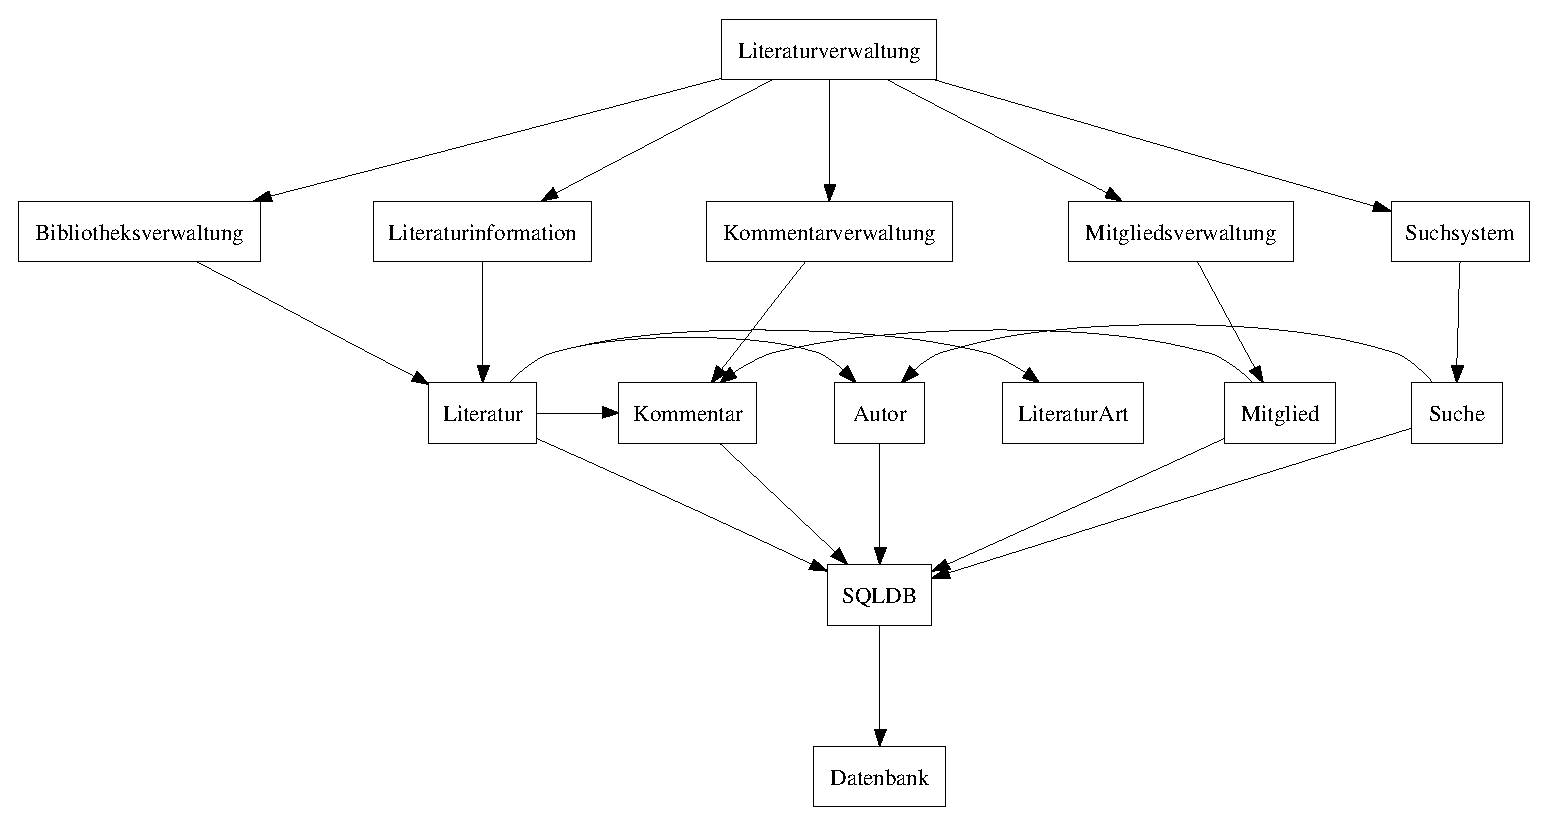
\includegraphics[scale=0.56]{systemarchitektur}

Aus Gründen der Übersichtlichkeit wurde die Login-Hilfsklasse entfernt. Eine komplette Übersicht über die Klassen inklusive der Login-Hilfsklasse ist im Klassendiagramm möglich.
\clearpage
\section{Klassenspezifikation}
\hypertarget{classAutor}{
\subsection{Autor Klassenreferenz}
\label{classAutor}\index{Autor@{Autor}}
}
TODO.  


\subsubsection*{\"{O}ffentliche Methoden}
\begin{CompactItemize}
\item 
\hyperlink{classAutor_2302710dd8970853f5d49c62d4586e8f}{Autor} (\$data)
\begin{CompactList}\small\item\em TODO. \item\end{CompactList}\item 
\hyperlink{classAutor_77b27af7e471abe5a404fc92c7319921}{Clean} ()
\begin{CompactList}\small\item\em TODO. \item\end{CompactList}\item 
\hyperlink{classAutor_2ba5418b6622f414fa8a054e6c2a2db8}{Split} (\$autoren)
\begin{CompactList}\small\item\em TODO. \item\end{CompactList}\end{CompactItemize}
\subsubsection*{\"{O}ffentliche Attribute}
\begin{CompactItemize}
\item 
\hyperlink{classAutor_23e64634d5dc31b41b7ee9c49b9ea6b9}{\$Nr} = 0
\begin{CompactList}\small\item\em TODO. \item\end{CompactList}\item 
\hyperlink{classAutor_8602b5705cef83e7c16f4040f9add56d}{\$Name} = 0
\begin{CompactList}\small\item\em TODO. \item\end{CompactList}\end{CompactItemize}


\subsubsection{Ausf\"{u}hrliche Beschreibung}
TODO. 

TODO 



\subsubsection{Beschreibung der Konstruktoren und Destruktoren}
\hypertarget{classAutor_2302710dd8970853f5d49c62d4586e8f}{
\index{Autor@{Autor}!Autor@{Autor}}
\index{Autor@{Autor}!Autor@{Autor}}
\paragraph[Autor]{\setlength{\rightskip}{0pt plus 5cm}Autor::Autor (\$ {\em data})}\hfill}
\label{classAutor_2302710dd8970853f5d49c62d4586e8f}


TODO. 

TODO \begin{Desc}
\item[Vorbedingung:]TODO \end{Desc}
\begin{Desc}
\item[Parameter:]
\begin{description}
\item[\mbox{$\leftarrow$} {\em \$data}]TODO \end{description}
\end{Desc}


\subsubsection{Dokumentation der Elementfunktionen}
\hypertarget{classAutor_77b27af7e471abe5a404fc92c7319921}{
\index{Autor@{Autor}!Clean@{Clean}}
\index{Clean@{Clean}!Autor@{Autor}}
\paragraph[Clean]{\setlength{\rightskip}{0pt plus 5cm}Autor::Clean ()}\hfill}
\label{classAutor_77b27af7e471abe5a404fc92c7319921}


TODO. 

TODO \begin{Desc}
\item[Vorbedingung:]TODO \end{Desc}
\hypertarget{classAutor_2ba5418b6622f414fa8a054e6c2a2db8}{
\index{Autor@{Autor}!Split@{Split}}
\index{Split@{Split}!Autor@{Autor}}
\paragraph[Split]{\setlength{\rightskip}{0pt plus 5cm}Autor::Split (\$ {\em autoren})}\hfill}
\label{classAutor_2ba5418b6622f414fa8a054e6c2a2db8}


TODO. 

TODO \begin{Desc}
\item[Vorbedingung:]TODO \end{Desc}
\begin{Desc}
\item[Parameter:]
\begin{description}
\item[\mbox{$\leftarrow$} {\em \$autoren}]TODO \end{description}
\end{Desc}
\begin{Desc}
\item[R\"{u}ckgabe:]TODO \end{Desc}


\subsubsection{Dokumentation der Datenelemente}
\hypertarget{classAutor_8602b5705cef83e7c16f4040f9add56d}{
\index{Autor@{Autor}!$Name@{\$Name}}
\index{$Name@{\$Name}!Autor@{Autor}}
\paragraph[\$Name]{\setlength{\rightskip}{0pt plus 5cm}Autor::\$Name = 0}\hfill}
\label{classAutor_8602b5705cef83e7c16f4040f9add56d}


TODO. 

\hypertarget{classAutor_23e64634d5dc31b41b7ee9c49b9ea6b9}{
\index{Autor@{Autor}!$Nr@{\$Nr}}
\index{$Nr@{\$Nr}!Autor@{Autor}}
\paragraph[\$Nr]{\setlength{\rightskip}{0pt plus 5cm}Autor::\$Nr = 0}\hfill}
\label{classAutor_23e64634d5dc31b41b7ee9c49b9ea6b9}


TODO. 


\hypertarget{classKommentar}{
\subsection{Kommentar Klassenreferenz}
\label{classKommentar}\index{Kommentar@{Kommentar}}
}
Verwaltet Kommentare.  


\subsubsection*{\"{O}ffentliche Methoden}
\begin{CompactItemize}
\item 
\hyperlink{classKommentar_ea774e2108c754890c602dfdd53d64e1}{Kommentar} (\$data)
\begin{CompactList}\small\item\em Legt Kommentarobjekt an. \item\end{CompactList}\item 
\hyperlink{classKommentar_31c1fdfb4fb8f24e0016c8ddb98ddcdc}{Delete} (\$nr)
\begin{CompactList}\small\item\em Löscht \hyperlink{classKommentar}{Kommentar}. \item\end{CompactList}\item 
\hyperlink{classKommentar_9903f1df98f71eefa3b44a81d6a8ee5c}{Delete\-All} (\$literatur\_\-nr)
\begin{CompactList}\small\item\em Löscht alle zu einer \hyperlink{classLiteratur}{Literatur} gehörenden Kommentare. \item\end{CompactList}\item 
\hyperlink{classKommentar_92a8fcea1b065341c7c53e8a8464fcf0}{Delete\-All\-Member} (\$member\_\-nr)
\begin{CompactList}\small\item\em Löscht alle zu einem \hyperlink{classMitglied}{Mitglied} gehörenden Kommentare. \item\end{CompactList}\item 
\hyperlink{classKommentar_33d65db8c526c50017a5fa029bc04416}{Get\-All} (\$literatur\_\-nr)
\begin{CompactList}\small\item\em Gibt Kommentare zu bestimmter \hyperlink{classLiteratur}{Literatur} zurück. \item\end{CompactList}\item 
\hyperlink{classKommentar_6119b3c12a61d8d5a41cded165517914}{Insert} (\$text, \$verfasser\_\-nr, \$literatur\_\-nr)
\begin{CompactList}\small\item\em Legt \hyperlink{classKommentar}{Kommentar} an. \item\end{CompactList}\item 
\hyperlink{classKommentar_0b3e20e910493e67b67b747243f04511}{Update} (\$nr, \$text)
\begin{CompactList}\small\item\em Ändert einen \hyperlink{classKommentar}{Kommentar}. \item\end{CompactList}\end{CompactItemize}
\subsubsection*{\"{O}ffentliche Attribute}
\begin{CompactItemize}
\item 
\hyperlink{classKommentar_1b0a3cfcb9fc7075f985cc8067ab1982}{\$Nr}
\begin{CompactList}\small\item\em Identifikationsnummer des Kommentars. \item\end{CompactList}\item 
\hyperlink{classKommentar_c9a481413d6ba0c000719ad514bad4b5}{\$Text}
\begin{CompactList}\small\item\em Kommentartext. \item\end{CompactList}\item 
\hyperlink{classKommentar_c92b002e40690ee052fec446ff2a0ef6}{\$Verfasser\_\-Nr}
\begin{CompactList}\small\item\em Mitglieds\_\-Nr des Verfassers. \item\end{CompactList}\item 
\hyperlink{classKommentar_84f0fc10295968adde28169f8df018d9}{\$Verfasser\_\-Name}
\begin{CompactList}\small\item\em Name des Verfassers (Vor- und Nachname). \item\end{CompactList}\end{CompactItemize}


\subsubsection{Ausf\"{u}hrliche Beschreibung}
Verwaltet Kommentare. 

Stellt Funktionen zum Anlegen, Löschen, Bearbeiten von Kommentaren bereit. Es können sowohl einzelne Kommentare oder Kommentare nach ihrer Verbindung zur \hyperlink{classLiteratur}{Literatur} bzw. Mitgliedern gelöscht werden. \begin{Desc}
\item[Vorbedingung:]Datenbankverbindung muss bestehen \end{Desc}
\begin{Desc}
\item[Importiert:]\begin{itemize}
\item \hyperlink{classLogin_6c120224aa6719f58c6ccd08acc28758}{Login::Is\-Administrator}\item \hyperlink{classLogin_70d2747b0aa454f4203a789afea25318}{Login::Is\-Member}\item \hyperlink{classSQLDB_fc6ffa8df50f68f07d9f5e3385b96d7a}{SQLDB::Query}\item \hyperlink{classSQLDB_a55c00ce1de0e50e0a58cae61892ba35}{SQLDB::Fetch}\end{itemize}
\end{Desc}
\begin{Desc}
\item[Autor:]Frank Wilhelm \end{Desc}
\begin{Desc}
\item[Änderungsstand:]30.05.2006 \end{Desc}




\subsubsection{Beschreibung der Konstruktoren und Destruktoren}
\hypertarget{classKommentar_ea774e2108c754890c602dfdd53d64e1}{
\index{Kommentar@{Kommentar}!Kommentar@{Kommentar}}
\index{Kommentar@{Kommentar}!Kommentar@{Kommentar}}
\paragraph[Kommentar]{\setlength{\rightskip}{0pt plus 5cm}Kommentar::Kommentar (\$ {\em data})}\hfill}
\label{classKommentar_ea774e2108c754890c602dfdd53d64e1}


Legt Kommentarobjekt an. 

Legt ein neues Kommentarobjekt aus einem Objekt mit den Attributen Nr, Text, Verfasser\_\-Nr und Verfasser\_\-Name an. \begin{Desc}
\item[Vorbedingung:]- \end{Desc}
\begin{Desc}
\item[Parameter:]
\begin{description}
\item[\mbox{$\leftarrow$} {\em \$data}]Objekt mit Kommentardaten der Form\begin{itemize}
\item Nr\item Text\item Mitglieds\_\-Nr\item Vorname\item Nachname \end{itemize}
\end{description}
\end{Desc}


\subsubsection{Dokumentation der Elementfunktionen}
\hypertarget{classKommentar_31c1fdfb4fb8f24e0016c8ddb98ddcdc}{
\index{Kommentar@{Kommentar}!Delete@{Delete}}
\index{Delete@{Delete}!Kommentar@{Kommentar}}
\paragraph[Delete]{\setlength{\rightskip}{0pt plus 5cm}Kommentar::Delete (\$ {\em nr})}\hfill}
\label{classKommentar_31c1fdfb4fb8f24e0016c8ddb98ddcdc}


Löscht \hyperlink{classKommentar}{Kommentar}. 

Löscht einen \hyperlink{classKommentar}{Kommentar} aus Kommentare mit der Kommentar\_\-Nr \$nr. \begin{Desc}
\item[Vorbedingung:]Datenbankverbindung muss bestehen 

\hyperlink{classKommentar}{Kommentar} in Kommentare mit Kommentar\_\-Nr \$nr muss existieren \end{Desc}
\begin{Desc}
\item[Parameter:]
\begin{description}
\item[\mbox{$\leftarrow$} {\em \$nr}]Nummer des zu löschenden Kommentars \end{description}
\end{Desc}
\begin{Desc}
\item[Bemerkungen:]Ist der Nutzer nicht als Administrator angemeldet, werden keine Operationen ausgeführt, wenn Mitglieds\_\-Nr des Kommentars ungleich der eigenen Mitglieds\_\-Nr ist. Ist der Nutzer nicht angemeldet, werden keine Operationen ausgeführt \end{Desc}
\hypertarget{classKommentar_9903f1df98f71eefa3b44a81d6a8ee5c}{
\index{Kommentar@{Kommentar}!DeleteAll@{DeleteAll}}
\index{DeleteAll@{DeleteAll}!Kommentar@{Kommentar}}
\paragraph[DeleteAll]{\setlength{\rightskip}{0pt plus 5cm}Kommentar::Delete\-All (\$ {\em literatur\_\-nr})}\hfill}
\label{classKommentar_9903f1df98f71eefa3b44a81d6a8ee5c}


Löscht alle zu einer \hyperlink{classLiteratur}{Literatur} gehörenden Kommentare. 

Löscht alle Kommentare aus Kommentare, die mit \hyperlink{classLiteratur}{Literatur} mit der Literaturnummer (\$literatur\_\-nr) verbunden sind. \begin{Desc}
\item[Vorbedingung:]Datenbankverbindung muss bestehen \end{Desc}
\begin{Desc}
\item[Parameter:]
\begin{description}
\item[\mbox{$\leftarrow$} {\em \$literatur\_\-nr}]Nummer der \hyperlink{classLiteratur}{Literatur} \end{description}
\end{Desc}
\begin{Desc}
\item[Bemerkungen:]Ist Nutzer nicht eingeloggt, werden keine Operationen ausgeführt. \end{Desc}
\hypertarget{classKommentar_92a8fcea1b065341c7c53e8a8464fcf0}{
\index{Kommentar@{Kommentar}!DeleteAllMember@{DeleteAllMember}}
\index{DeleteAllMember@{DeleteAllMember}!Kommentar@{Kommentar}}
\paragraph[DeleteAllMember]{\setlength{\rightskip}{0pt plus 5cm}Kommentar::Delete\-All\-Member (\$ {\em member\_\-nr})}\hfill}
\label{classKommentar_92a8fcea1b065341c7c53e8a8464fcf0}


Löscht alle zu einem \hyperlink{classMitglied}{Mitglied} gehörenden Kommentare. 

Löscht alle Kommentare aus Kommentare, die mit Mitglieder mit der Mitglieds\_\-Nr (\$member\_\-nr) verbunden sind. \begin{Desc}
\item[Vorbedingung:]Datenbankverbindung muss bestehen \end{Desc}
\begin{Desc}
\item[Parameter:]
\begin{description}
\item[\mbox{$\leftarrow$} {\em \$member\_\-nr}]Nummer eines Mitglieds \end{description}
\end{Desc}
\begin{Desc}
\item[Bemerkungen:]Ist der Nutzer nicht als Administrator eingeloggt, werden keine Operationen ausgeführt. \end{Desc}
\hypertarget{classKommentar_33d65db8c526c50017a5fa029bc04416}{
\index{Kommentar@{Kommentar}!GetAll@{GetAll}}
\index{GetAll@{GetAll}!Kommentar@{Kommentar}}
\paragraph[GetAll]{\setlength{\rightskip}{0pt plus 5cm}Kommentar::Get\-All (\$ {\em literatur\_\-nr})}\hfill}
\label{classKommentar_33d65db8c526c50017a5fa029bc04416}


Gibt Kommentare zu bestimmter \hyperlink{classLiteratur}{Literatur} zurück. 

Liest alle Kommentare die einer \hyperlink{classLiteratur}{Literatur} (\$literatur\_\-nr) zugeordnet sind aus Kommentare aus und gibt sie als Feld des Typs \hyperlink{classKommentar}{Kommentar} zurück. \begin{Desc}
\item[Parameter:]
\begin{description}
\item[\mbox{$\leftarrow$} {\em \$literatur\_\-nr}]Nr einer \hyperlink{classLiteratur}{Literatur} mit Kommentaren \end{description}
\end{Desc}
\begin{Desc}
\item[Vorbedingung:]Datenbankverbindung muss bestehen \end{Desc}
\begin{Desc}
\item[R\"{u}ckgabe:]Feld vom Typ \hyperlink{classKommentar}{Kommentar} \end{Desc}
\hypertarget{classKommentar_6119b3c12a61d8d5a41cded165517914}{
\index{Kommentar@{Kommentar}!Insert@{Insert}}
\index{Insert@{Insert}!Kommentar@{Kommentar}}
\paragraph[Insert]{\setlength{\rightskip}{0pt plus 5cm}Kommentar::Insert (\$ {\em text}, \$ {\em verfasser\_\-nr}, \$ {\em literatur\_\-nr})}\hfill}
\label{classKommentar_6119b3c12a61d8d5a41cded165517914}


Legt \hyperlink{classKommentar}{Kommentar} an. 

Legt einen neuen \hyperlink{classKommentar}{Kommentar} mit Text (\$text) zu einer \hyperlink{classLiteratur}{Literatur} (\$literatur\_\-nr) vom einem Verfasser (\$verfasser\_\-nr) an. \begin{Desc}
\item[Vorbedingung:]Datenbankverbindung muss bestehen 

Text (\$text) darf nicht leer sein \end{Desc}
\begin{Desc}
\item[Parameter:]
\begin{description}
\item[\mbox{$\leftarrow$} {\em \$text}]Text des Kommentars \item[\mbox{$\leftarrow$} {\em \$verfasser\_\-nr}]Mitglieds\_\-Nr des Verfassers \item[\mbox{$\leftarrow$} {\em \$literatur\_\-nr}]Nummer der \hyperlink{classLiteratur}{Literatur} \end{description}
\end{Desc}
\begin{Desc}
\item[Bemerkungen:]Ist das aktuelle \hyperlink{classMitglied}{Mitglied} kein Administrator, dann muss \$verfasser\_\-nr gleich der aktuellen Nummer des Logins sein. Ist der Nutzer nicht eingeloggt, werden keine Operationen ausgeführt. Ist keine passende \hyperlink{classLiteratur}{Literatur} mit der Literatur\_\-Nr \$literatur\_\-nr vorhanden, wird kein \hyperlink{classKommentar}{Kommentar} angelegt. Existiert schon ein \hyperlink{classKommentar}{Kommentar} zu \hyperlink{classLiteratur}{Literatur} mit \$literatur\_\-nr von \hyperlink{classMitglied}{Mitglied} mit Mitglieds\_\-Nr \$verfasser\_\-nr, wird nur der Text des Kommentars mit \hyperlink{classKommentar_0b3e20e910493e67b67b747243f04511}{Kommentar::Update} geändert. \end{Desc}
\hypertarget{classKommentar_0b3e20e910493e67b67b747243f04511}{
\index{Kommentar@{Kommentar}!Update@{Update}}
\index{Update@{Update}!Kommentar@{Kommentar}}
\paragraph[Update]{\setlength{\rightskip}{0pt plus 5cm}Kommentar::Update (\$ {\em nr}, \$ {\em text})}\hfill}
\label{classKommentar_0b3e20e910493e67b67b747243f04511}


Ändert einen \hyperlink{classKommentar}{Kommentar}. 

Ändert in Kommentare den Text des Kommentars mit \$nr in \$text. \begin{Desc}
\item[Vorbedingung:]Datenbankverbindung muss bestehen 

\hyperlink{classKommentar}{Kommentar} in Kommentare mit Kommentar\_\-Nr \$nr muss existieren \end{Desc}
\begin{Desc}
\item[Parameter:]
\begin{description}
\item[\mbox{$\leftarrow$} {\em \$nr}]Nummer des zu verändernden Kommentars \item[\mbox{$\leftarrow$} {\em \$text}]neuer Text des Kommentars \end{description}
\end{Desc}
\begin{Desc}
\item[Bemerkungen:]Ist das aktuelle \hyperlink{classMitglied}{Mitglied} kein Administrator, dann muss die aktuelle Nummer des Mitglieds gleich der Mitglieds\_\-Nr des Kommentars in Kommentare sein. Ist der Nutzer nicht eingeloggt, werden keine Operationen ausgeführt. Wird kein Text (\$text) angegeben, wird der \hyperlink{classKommentar}{Kommentar} mit \hyperlink{classKommentar_31c1fdfb4fb8f24e0016c8ddb98ddcdc}{Kommentar::Delete} gelöscht. \end{Desc}


\subsubsection{Dokumentation der Datenelemente}
\hypertarget{classKommentar_1b0a3cfcb9fc7075f985cc8067ab1982}{
\index{Kommentar@{Kommentar}!$Nr@{\$Nr}}
\index{$Nr@{\$Nr}!Kommentar@{Kommentar}}
\paragraph[\$Nr]{\setlength{\rightskip}{0pt plus 5cm}Kommentar::\$Nr}\hfill}
\label{classKommentar_1b0a3cfcb9fc7075f985cc8067ab1982}


Identifikationsnummer des Kommentars. 

\hypertarget{classKommentar_c9a481413d6ba0c000719ad514bad4b5}{
\index{Kommentar@{Kommentar}!$Text@{\$Text}}
\index{$Text@{\$Text}!Kommentar@{Kommentar}}
\paragraph[\$Text]{\setlength{\rightskip}{0pt plus 5cm}Kommentar::\$Text}\hfill}
\label{classKommentar_c9a481413d6ba0c000719ad514bad4b5}


Kommentartext. 

\hypertarget{classKommentar_84f0fc10295968adde28169f8df018d9}{
\index{Kommentar@{Kommentar}!$Verfasser_Name@{\$Verfasser\_\-Name}}
\index{$Verfasser_Name@{\$Verfasser\_\-Name}!Kommentar@{Kommentar}}
\paragraph[\$Verfasser\_\-Name]{\setlength{\rightskip}{0pt plus 5cm}Kommentar::\$Verfasser\_\-Name}\hfill}
\label{classKommentar_84f0fc10295968adde28169f8df018d9}


Name des Verfassers (Vor- und Nachname). 

\hypertarget{classKommentar_c92b002e40690ee052fec446ff2a0ef6}{
\index{Kommentar@{Kommentar}!$Verfasser_Nr@{\$Verfasser\_\-Nr}}
\index{$Verfasser_Nr@{\$Verfasser\_\-Nr}!Kommentar@{Kommentar}}
\paragraph[\$Verfasser\_\-Nr]{\setlength{\rightskip}{0pt plus 5cm}Kommentar::\$Verfasser\_\-Nr}\hfill}
\label{classKommentar_c92b002e40690ee052fec446ff2a0ef6}


Mitglieds\_\-Nr des Verfassers. 


\hypertarget{classLiteratur}{
\subsection{Literatur Klassenreferenz}
\label{classLiteratur}\index{Literatur@{Literatur}}
}
Verwaltet \hyperlink{classLiteratur}{Literatur}.  


\subsubsection*{\"{O}ffentliche Methoden}
\begin{CompactItemize}
\item 
\hyperlink{classLiteratur_55626b912da4c041eaf981781ed6c640}{Literatur} (\$nr)
\begin{CompactList}\small\item\em Liest \hyperlink{classLiteratur}{Literatur} ein. \item\end{CompactList}\item 
\hyperlink{classLiteratur_11f6d1a4409c41638ff6693f65699ff3}{To\-Bibtex} ()
\begin{CompactList}\small\item\em Exportiert \hyperlink{classLiteratur}{Literatur} nach \hyperlink{classBibTeX}{Bib\-Te\-X}. \item\end{CompactList}\item 
\hyperlink{classLiteratur_f5b265d349df2a9d17079b81d808fa89}{Delete} (\$nr)
\begin{CompactList}\small\item\em Löscht \hyperlink{classLiteratur}{Literatur}. \item\end{CompactList}\item 
\hyperlink{classLiteratur_d466a307b1971ee736e1d4ba9342dc55}{Insert\-Bib\-Te\-X} (\$bibtex)
\begin{CompactList}\small\item\em Importiert \hyperlink{classBibTeX}{Bib\-Te\-X}. \item\end{CompactList}\item 
\hyperlink{classLiteratur_3347551316e8f73659fc6f32ac6095df}{Insert} (\$autoren, \$art, \$titel, \$jahr, \$verlag, \$isbn, \$beschreibung, \$ort, \$stichworte)
\begin{CompactList}\small\item\em Legt \hyperlink{classLiteratur}{Literatur} an. \item\end{CompactList}\item 
\hyperlink{classLiteratur_b613c28476ea28058f8fc2bccb57c923}{Update} (\$nr, \$autoren, \$art, \$titel, \$jahr, \$verlag, \$isbn, \$beschreibung, \$ort, \$stichworte)
\begin{CompactList}\small\item\em Ändert \hyperlink{classLiteratur}{Literatur}. \item\end{CompactList}\end{CompactItemize}
\subsubsection*{\"{O}ffentliche Attribute}
\begin{CompactItemize}
\item 
\hyperlink{classLiteratur_036a682a93a5d50839c1ebc70a79d4b6}{\$Nr}
\begin{CompactList}\small\item\em Literaturidentifikationsnummer. \item\end{CompactList}\item 
\hyperlink{classLiteratur_e30f9e9db9b396e6f87adfdb94e12ba0}{\$Titel}
\begin{CompactList}\small\item\em Titel der \hyperlink{classLiteratur}{Literatur}. \item\end{CompactList}\item 
\hyperlink{classLiteratur_2cb6f40a8757a0edd5da32385ad009c9}{\$Jahr}
\begin{CompactList}\small\item\em Erscheinungsjahr. \item\end{CompactList}\item 
\hyperlink{classLiteratur_5f591208e5d21bb81e6c51484e2a60e0}{\$Verlag}
\begin{CompactList}\small\item\em Verlag/Herausgeber. \item\end{CompactList}\item 
\hyperlink{classLiteratur_9e3b00766297a68adac423980767dd3c}{\$ISBN}
\begin{CompactList}\small\item\em ISBN der \hyperlink{classLiteratur}{Literatur}. \item\end{CompactList}\item 
\hyperlink{classLiteratur_6769ff8b353d2f789125f009b4dcfdc0}{\$Beschreibung}
\begin{CompactList}\small\item\em Bemerkung zur \hyperlink{classLiteratur}{Literatur}. \item\end{CompactList}\item 
\hyperlink{classLiteratur_da6c458bb229187efea8e8f144a1d279}{\$Ort}
\begin{CompactList}\small\item\em Herausgabeort. \item\end{CompactList}\item 
\hyperlink{classLiteratur_aa77f0f697d4bcf72279aadedd91ddff}{\$Stichworte}
\begin{CompactList}\small\item\em Stichworte zum Inhalt der \hyperlink{classLiteratur}{Literatur}. \item\end{CompactList}\item 
\hyperlink{classLiteratur_fb4d4b1ce29a33a10e3e27d47f31a447}{\$Art}
\begin{CompactList}\small\item\em Typ der \hyperlink{classLiteratur}{Literatur}. \item\end{CompactList}\item 
\hyperlink{classLiteratur_01b311917d78c1dbb346435598ebba64}{\$Autoren}
\begin{CompactList}\small\item\em Feld mit Autoren der \hyperlink{classLiteratur}{Literatur}. \item\end{CompactList}\item 
\hyperlink{classLiteratur_ebcaeb5c38ce2677a14189da511fa663}{\$Kommentare}
\begin{CompactList}\small\item\em Feld mit Kommentaren der \hyperlink{classLiteratur}{Literatur}. \item\end{CompactList}\end{CompactItemize}


\subsubsection{Ausf\"{u}hrliche Beschreibung}
Verwaltet \hyperlink{classLiteratur}{Literatur}. 

Stellt Funktionen zum Abruf, Exportieren, Löschen, Importieren, Hinzufügen und Ändern von \hyperlink{classLiteratur}{Literatur} in Bibliothek zur Verfügung. \begin{Desc}
\item[Vorbedingung:]Datenbankverbindung muss bestehen \end{Desc}
\begin{Desc}
\item[Importiert:]\begin{itemize}
\item \hyperlink{classAutor_77b27af7e471abe5a404fc92c7319921}{Autor::Clean}\item \hyperlink{classAutor_79cd90084cab240919a5daecf39156a7}{Autor::Get\-All}\item \hyperlink{classAutor_2ba5418b6622f414fa8a054e6c2a2db8}{Autor::Split}\item \hyperlink{classKommentar_9903f1df98f71eefa3b44a81d6a8ee5c}{Kommentar::Delete\-All}\item \hyperlink{classKommentar_33d65db8c526c50017a5fa029bc04416}{Kommentar::Get\-All}\item \hyperlink{classLiteraturArt_b3312217430531ed7821a46a39c49af7}{Literatur\-Art::Literatur\-Art}\item Literatur\-Art::Get\-Bib\-Tex\-Text\item \hyperlink{classLogin_70d2747b0aa454f4203a789afea25318}{Login::Is\-Member}\item \hyperlink{classSQLDB_fc6ffa8df50f68f07d9f5e3385b96d7a}{SQLDB::Query}\item \hyperlink{classSQLDB_a55c00ce1de0e50e0a58cae61892ba35}{SQLDB::Fetch}\end{itemize}
\end{Desc}
\begin{Desc}
\item[Autor:]Sven Eckelmann \end{Desc}
\begin{Desc}
\item[Änderungsstand:]30.05.2006 \end{Desc}




\subsubsection{Beschreibung der Konstruktoren und Destruktoren}
\hypertarget{classLiteratur_55626b912da4c041eaf981781ed6c640}{
\index{Literatur@{Literatur}!Literatur@{Literatur}}
\index{Literatur@{Literatur}!Literatur@{Literatur}}
\paragraph[Literatur]{\setlength{\rightskip}{0pt plus 5cm}Literatur::Literatur (\$ {\em nr})}\hfill}
\label{classLiteratur_55626b912da4c041eaf981781ed6c640}


Liest \hyperlink{classLiteratur}{Literatur} ein. 

Erstellt aus \hyperlink{classLiteratur}{Literatur} in Bibliothek mit Literatur\_\-Nr (\$nr) neues Literaturobjekt. \begin{Desc}
\item[Vorbedingung:]Datenbankverbindung muss bestehen 

\hyperlink{classLiteratur}{Literatur} in Bibliothek mit Literatur\_\-Nr \$nr muss existieren \end{Desc}
\begin{Desc}
\item[Parameter:]
\begin{description}
\item[\mbox{$\leftarrow$} {\em \$nr}]Nummer der zu einlesenden \hyperlink{classLiteratur}{Literatur} \end{description}
\end{Desc}


\subsubsection{Dokumentation der Elementfunktionen}
\hypertarget{classLiteratur_f5b265d349df2a9d17079b81d808fa89}{
\index{Literatur@{Literatur}!Delete@{Delete}}
\index{Delete@{Delete}!Literatur@{Literatur}}
\paragraph[Delete]{\setlength{\rightskip}{0pt plus 5cm}Literatur::Delete (\$ {\em nr})}\hfill}
\label{classLiteratur_f5b265d349df2a9d17079b81d808fa89}


Löscht \hyperlink{classLiteratur}{Literatur}. 

Löscht \hyperlink{classLiteratur}{Literatur} aus Bibliothek mit der Literatur\_\-Nr \$nr. Alle verbundenen Kommentare werden aus Kommentare gelöscht. Außerdem werden alle nun nicht mehr gebrauchten Autoren in Autoren gelöscht. \begin{Desc}
\item[Vorbedingung:]Datenbankverbindung muss bestehen 

\hyperlink{classLiteratur}{Literatur} in Bibliothek mit Literatur\_\-Nr \$nr muss existieren \end{Desc}
\begin{Desc}
\item[Parameter:]
\begin{description}
\item[\mbox{$\leftarrow$} {\em \$nr}]Nummer der zu löschenden \hyperlink{classLiteratur}{Literatur} \end{description}
\end{Desc}
\begin{Desc}
\item[Bemerkungen:]Ist der Nutzer nicht als \hyperlink{classMitglied}{Mitglied} angemeldet, werden keine Operationen ausgeführt \end{Desc}
\hypertarget{classLiteratur_3347551316e8f73659fc6f32ac6095df}{
\index{Literatur@{Literatur}!Insert@{Insert}}
\index{Insert@{Insert}!Literatur@{Literatur}}
\paragraph[Insert]{\setlength{\rightskip}{0pt plus 5cm}Literatur::Insert (\$ {\em autoren}, \$ {\em art}, \$ {\em titel}, \$ {\em jahr}, \$ {\em verlag}, \$ {\em isbn}, \$ {\em beschreibung}, \$ {\em ort}, \$ {\em stichworte})}\hfill}
\label{classLiteratur_3347551316e8f73659fc6f32ac6095df}


Legt \hyperlink{classLiteratur}{Literatur} an. 

Legt neue \hyperlink{classLiteratur}{Literatur} in Bibliothek mit den übergebenen Parametern (\$art, \$titel, \$jahr, \$verlag, \$isbn, \$beschreibung, \$ort, \$stichworte) an. Danach werden die Autoren (\$autoren) in Autoren geschrieben und mit der Tabelle Literatur\_\-Autor der \hyperlink{classLiteratur}{Literatur} zugeordnet. \begin{Desc}
\item[Vorbedingung:]Datenbankverbindung muss bestehen \end{Desc}
\begin{Desc}
\item[Parameter:]
\begin{description}
\item[\mbox{$\leftarrow$} {\em \$autoren}]String mit kommagetrennter Liste von Autoren \item[\mbox{$\leftarrow$} {\em \$art}]Bezeichner der Literaturart \item[\mbox{$\leftarrow$} {\em \$titel}]Titel der \hyperlink{classLiteratur}{Literatur} \item[\mbox{$\leftarrow$} {\em \$jahr}]Erscheinungsjahr der \hyperlink{classLiteratur}{Literatur} \item[\mbox{$\leftarrow$} {\em \$verlag}]Verlag der \hyperlink{classLiteratur}{Literatur} \item[\mbox{$\leftarrow$} {\em \$isbn}]ISBN der \hyperlink{classLiteratur}{Literatur} \item[\mbox{$\leftarrow$} {\em \$beschreibung}]Beschreibung der \hyperlink{classLiteratur}{Literatur} \item[\mbox{$\leftarrow$} {\em \$ort}]Erscheinungsort \item[\mbox{$\leftarrow$} {\em \$stichworte}]Stichworte \end{description}
\end{Desc}
\begin{Desc}
\item[Bemerkungen:]Ist der Nutzer nicht als \hyperlink{classMitglied}{Mitglied} angemeldet, werden keine Operationen ausgeführt \end{Desc}
\hypertarget{classLiteratur_d466a307b1971ee736e1d4ba9342dc55}{
\index{Literatur@{Literatur}!InsertBibTeX@{InsertBibTeX}}
\index{InsertBibTeX@{InsertBibTeX}!Literatur@{Literatur}}
\paragraph[InsertBibTeX]{\setlength{\rightskip}{0pt plus 5cm}Literatur::Insert\-Bib\-Te\-X (\$ {\em bibtex})}\hfill}
\label{classLiteratur_d466a307b1971ee736e1d4ba9342dc55}


Importiert \hyperlink{classBibTeX}{Bib\-Te\-X}. 

Importiert \hyperlink{classLiteratur}{Literatur} nach Bibliothek aus einem Bib\-Te\-X-formatierten String. Alle Einträge werden dazu nacheinandere eingelesen und umgewandelt, um diese dann in die Datenbank zu schreiben. \begin{Desc}
\item[Vorbedingung:]Datenbankverbindung muss bestehen \end{Desc}
\begin{Desc}
\item[Parameter:]
\begin{description}
\item[\mbox{$\leftarrow$} {\em \$bibtex}]String mit Inhalt einer Bib\-Te\-X-Datei \end{description}
\end{Desc}
\begin{Desc}
\item[R\"{u}ckgabe:]Anzahl der importierten \hyperlink{classLiteratur}{Literatur}\end{Desc}
\hypertarget{classLiteratur_11f6d1a4409c41638ff6693f65699ff3}{
\index{Literatur@{Literatur}!ToBibtex@{ToBibtex}}
\index{ToBibtex@{ToBibtex}!Literatur@{Literatur}}
\paragraph[ToBibtex]{\setlength{\rightskip}{0pt plus 5cm}Literatur::To\-Bibtex ()}\hfill}
\label{classLiteratur_11f6d1a4409c41638ff6693f65699ff3}


Exportiert \hyperlink{classLiteratur}{Literatur} nach \hyperlink{classBibTeX}{Bib\-Te\-X}. 

Exportiert die aktuellen Informationen im Literaturobjekt in das Bib\-Te\-X-Format. \begin{Desc}
\item[Vorbedingung:]- \end{Desc}
\begin{Desc}
\item[R\"{u}ckgabe:]\$string mit Bib\-Te\-X-Eintrag \end{Desc}
\hypertarget{classLiteratur_b613c28476ea28058f8fc2bccb57c923}{
\index{Literatur@{Literatur}!Update@{Update}}
\index{Update@{Update}!Literatur@{Literatur}}
\paragraph[Update]{\setlength{\rightskip}{0pt plus 5cm}Literatur::Update (\$ {\em nr}, \$ {\em autoren}, \$ {\em art}, \$ {\em titel}, \$ {\em jahr}, \$ {\em verlag}, \$ {\em isbn}, \$ {\em beschreibung}, \$ {\em ort}, \$ {\em stichworte})}\hfill}
\label{classLiteratur_b613c28476ea28058f8fc2bccb57c923}


Ändert \hyperlink{classLiteratur}{Literatur}. 

Entfernt alle zur Literatur\_\-Nr (\$nr) gehörenden Verbindungen in Autor\_\-Literatur um danach die \hyperlink{classLiteratur}{Literatur} mit Literatur\_\-Nr \$nr zu den neuen Werten (\$art, \$titel, \$jahr, \$verlag, \$isbn, \$beschreibung, \$ort, \$stichworte) zu ändern. Danach werden die Autoren (\$autoren) in Autoren geschrieben und mit der Tabelle Literatur\_\-Autor der \hyperlink{classLiteratur}{Literatur} zugeordnet. Alle jetzt noch nicht zugeordneten Autoren in Autoren werden gelöscht. \begin{Desc}
\item[Vorbedingung:]Datenbankverbindung muss bestehen 

\hyperlink{classLiteratur}{Literatur} in Bibliothek mit Literatur\_\-Nr \$nr muss existieren \end{Desc}
\begin{Desc}
\item[Parameter:]
\begin{description}
\item[\mbox{$\leftarrow$} {\em \$nr}]Nummer der zu verändernden \hyperlink{classLiteratur}{Literatur} \item[\mbox{$\leftarrow$} {\em \$autoren}]String mit kommagetrennter Liste von Autoren \item[\mbox{$\leftarrow$} {\em \$art}]neuer Bezeichner der Literaturart \item[\mbox{$\leftarrow$} {\em \$titel}]neuer Titel der \hyperlink{classLiteratur}{Literatur} \item[\mbox{$\leftarrow$} {\em \$jahr}]neues Erscheinungsjahr der \hyperlink{classLiteratur}{Literatur} \item[\mbox{$\leftarrow$} {\em \$verlag}]neuer Verlag der \hyperlink{classLiteratur}{Literatur} \item[\mbox{$\leftarrow$} {\em \$isbn}]neue ISBN der \hyperlink{classLiteratur}{Literatur} \item[\mbox{$\leftarrow$} {\em \$beschreibung}]neue Beschreibung der \hyperlink{classLiteratur}{Literatur} \item[\mbox{$\leftarrow$} {\em \$ort}]neuer Erscheinungsort \item[\mbox{$\leftarrow$} {\em \$stichworte}]neue Stichworte \end{description}
\end{Desc}
\begin{Desc}
\item[Bemerkungen:]Ist der Nutzer nicht als \hyperlink{classMitglied}{Mitglied} angemeldet, werden keine Operationen ausgeführt \end{Desc}


\subsubsection{Dokumentation der Datenelemente}
\hypertarget{classLiteratur_fb4d4b1ce29a33a10e3e27d47f31a447}{
\index{Literatur@{Literatur}!$Art@{\$Art}}
\index{$Art@{\$Art}!Literatur@{Literatur}}
\paragraph[\$Art]{\setlength{\rightskip}{0pt plus 5cm}Literatur::\$Art}\hfill}
\label{classLiteratur_fb4d4b1ce29a33a10e3e27d47f31a447}


Typ der \hyperlink{classLiteratur}{Literatur}. 

\hypertarget{classLiteratur_01b311917d78c1dbb346435598ebba64}{
\index{Literatur@{Literatur}!$Autoren@{\$Autoren}}
\index{$Autoren@{\$Autoren}!Literatur@{Literatur}}
\paragraph[\$Autoren]{\setlength{\rightskip}{0pt plus 5cm}Literatur::\$Autoren}\hfill}
\label{classLiteratur_01b311917d78c1dbb346435598ebba64}


Feld mit Autoren der \hyperlink{classLiteratur}{Literatur}. 

\hypertarget{classLiteratur_6769ff8b353d2f789125f009b4dcfdc0}{
\index{Literatur@{Literatur}!$Beschreibung@{\$Beschreibung}}
\index{$Beschreibung@{\$Beschreibung}!Literatur@{Literatur}}
\paragraph[\$Beschreibung]{\setlength{\rightskip}{0pt plus 5cm}Literatur::\$Beschreibung}\hfill}
\label{classLiteratur_6769ff8b353d2f789125f009b4dcfdc0}


Bemerkung zur \hyperlink{classLiteratur}{Literatur}. 

\hypertarget{classLiteratur_9e3b00766297a68adac423980767dd3c}{
\index{Literatur@{Literatur}!$ISBN@{\$ISBN}}
\index{$ISBN@{\$ISBN}!Literatur@{Literatur}}
\paragraph[\$ISBN]{\setlength{\rightskip}{0pt plus 5cm}Literatur::\$ISBN}\hfill}
\label{classLiteratur_9e3b00766297a68adac423980767dd3c}


ISBN der \hyperlink{classLiteratur}{Literatur}. 

\hypertarget{classLiteratur_2cb6f40a8757a0edd5da32385ad009c9}{
\index{Literatur@{Literatur}!$Jahr@{\$Jahr}}
\index{$Jahr@{\$Jahr}!Literatur@{Literatur}}
\paragraph[\$Jahr]{\setlength{\rightskip}{0pt plus 5cm}Literatur::\$Jahr}\hfill}
\label{classLiteratur_2cb6f40a8757a0edd5da32385ad009c9}


Erscheinungsjahr. 

\hypertarget{classLiteratur_ebcaeb5c38ce2677a14189da511fa663}{
\index{Literatur@{Literatur}!$Kommentare@{\$Kommentare}}
\index{$Kommentare@{\$Kommentare}!Literatur@{Literatur}}
\paragraph[\$Kommentare]{\setlength{\rightskip}{0pt plus 5cm}Literatur::\$Kommentare}\hfill}
\label{classLiteratur_ebcaeb5c38ce2677a14189da511fa663}


Feld mit Kommentaren der \hyperlink{classLiteratur}{Literatur}. 

\hypertarget{classLiteratur_036a682a93a5d50839c1ebc70a79d4b6}{
\index{Literatur@{Literatur}!$Nr@{\$Nr}}
\index{$Nr@{\$Nr}!Literatur@{Literatur}}
\paragraph[\$Nr]{\setlength{\rightskip}{0pt plus 5cm}Literatur::\$Nr}\hfill}
\label{classLiteratur_036a682a93a5d50839c1ebc70a79d4b6}


Literaturidentifikationsnummer. 

\hypertarget{classLiteratur_da6c458bb229187efea8e8f144a1d279}{
\index{Literatur@{Literatur}!$Ort@{\$Ort}}
\index{$Ort@{\$Ort}!Literatur@{Literatur}}
\paragraph[\$Ort]{\setlength{\rightskip}{0pt plus 5cm}Literatur::\$Ort}\hfill}
\label{classLiteratur_da6c458bb229187efea8e8f144a1d279}


Herausgabeort. 

\hypertarget{classLiteratur_aa77f0f697d4bcf72279aadedd91ddff}{
\index{Literatur@{Literatur}!$Stichworte@{\$Stichworte}}
\index{$Stichworte@{\$Stichworte}!Literatur@{Literatur}}
\paragraph[\$Stichworte]{\setlength{\rightskip}{0pt plus 5cm}Literatur::\$Stichworte}\hfill}
\label{classLiteratur_aa77f0f697d4bcf72279aadedd91ddff}


Stichworte zum Inhalt der \hyperlink{classLiteratur}{Literatur}. 

\hypertarget{classLiteratur_e30f9e9db9b396e6f87adfdb94e12ba0}{
\index{Literatur@{Literatur}!$Titel@{\$Titel}}
\index{$Titel@{\$Titel}!Literatur@{Literatur}}
\paragraph[\$Titel]{\setlength{\rightskip}{0pt plus 5cm}Literatur::\$Titel}\hfill}
\label{classLiteratur_e30f9e9db9b396e6f87adfdb94e12ba0}


Titel der \hyperlink{classLiteratur}{Literatur}. 

\hypertarget{classLiteratur_5f591208e5d21bb81e6c51484e2a60e0}{
\index{Literatur@{Literatur}!$Verlag@{\$Verlag}}
\index{$Verlag@{\$Verlag}!Literatur@{Literatur}}
\paragraph[\$Verlag]{\setlength{\rightskip}{0pt plus 5cm}Literatur::\$Verlag}\hfill}
\label{classLiteratur_5f591208e5d21bb81e6c51484e2a60e0}


Verlag/Herausgeber. 


\hypertarget{classLogin}{
\subsection{Login Klassenreferenz}
\label{classLogin}\index{Login@{Login}}
}
Verwaltet Logininformationen.  


\subsubsection*{\"{O}ffentliche Methoden}
\begin{CompactItemize}
\item 
\hyperlink{classLogin_4847f3e07e43b540d3339392346f87ff}{Login} ()
\begin{CompactList}\small\item\em Liest Session für Anmeldedaten ein. \item\end{CompactList}\item 
\hyperlink{classLogin_86b5c73ef1fb4bd03f91cc4771c960b7}{Login} (\$benutzer, \$passwort)
\begin{CompactList}\small\item\em Ändert Session mit neuen Anmeldedaten. \item\end{CompactList}\item 
\hyperlink{classLogin_4cbf74bd382f34e863aec07c3eda0400}{Logout} ()
\begin{CompactList}\small\item\em Entfernt Session. \item\end{CompactList}\item 
\hyperlink{classLogin_6c120224aa6719f58c6ccd08acc28758}{Is\-Administrator} ()
\begin{CompactList}\small\item\em Ermittelt ob Administratorrechte vorliegen. \item\end{CompactList}\item 
\hyperlink{classLogin_70d2747b0aa454f4203a789afea25318}{Is\-Member} ()
\begin{CompactList}\small\item\em Ermittelt ob mindestens Mitgliedsrechte vorliegen. \item\end{CompactList}\end{CompactItemize}


\subsubsection{Ausf\"{u}hrliche Beschreibung}
Verwaltet Logininformationen. 

Verwaltet die aus der sich aktuellen Anmeldung ergebenen Session des Users und der damit entstehenden Rechte \begin{Desc}
\item[Vorbedingung:]Das Loginobjekt muss vor einer Übertragung von Inhaltsdaten zum User angelegt werden, um ein Cookie anlegen zu können. Es sollte kein zweites Objekt vom Typ \hyperlink{classLogin}{Login} existieren. \end{Desc}
\begin{Desc}
\item[Bemerkungen:]Sollte ein weiteres Objekt vom Typ \hyperlink{classLogin}{Login} existieren, in welche neue Logininformationen eingetragen werden, wird keine weitere Session angelegt, sondern die alten Informationen in der aktuellen Session überschrieben. \end{Desc}




\subsubsection{Beschreibung der Konstruktoren und Destruktoren}
\hypertarget{classLogin_4847f3e07e43b540d3339392346f87ff}{
\index{Login@{Login}!Login@{Login}}
\index{Login@{Login}!Login@{Login}}
\paragraph[Login]{\setlength{\rightskip}{0pt plus 5cm}Login::Login ()}\hfill}
\label{classLogin_4847f3e07e43b540d3339392346f87ff}


Liest Session für Anmeldedaten ein. 

Liest Daten aus der Session ein. Sollten keine vorhanden sein, dann wird eine neue, leere Session angelegt. Sollten Daten vorhanden sein, wird die Korrektheit über die Datenbank (Mitglieder) und die Verbindungsinformationen geprüft. Nach dieser Prüfung werden abhängig vom Ausgang die Rechteinformationen gesetzt \begin{Desc}
\item[Vorbedingung:]Eine Verbindung zur Datenbank muss bestehen. Der Konstruktor muss vor dem Senden von Inhaltsdaten aufgerufen werden, um ein Cookie erstellen zu können. \end{Desc}
\hypertarget{classLogin_86b5c73ef1fb4bd03f91cc4771c960b7}{
\index{Login@{Login}!Login@{Login}}
\index{Login@{Login}!Login@{Login}}
\paragraph[Login]{\setlength{\rightskip}{0pt plus 5cm}Login::Login (\$ {\em benutzer}, \$ {\em passwort})}\hfill}
\label{classLogin_86b5c73ef1fb4bd03f91cc4771c960b7}


Ändert Session mit neuen Anmeldedaten. 

Das Klartextpasswort wird mit \hyperlink{classMitglied_9b13db80866c22bf992e73f2eb75e369}{Mitglied::Password\-Hash} gehasht, um diese mit Benutzernamen (\$benutzer) gegen die Einträge in Mitglieder zu prüfen. Ist diese erfolgreich, wird eine neue Session mit gehashtem Passwort, Benuternamen und Verbindungsinformationen erstellt. Sollte irgendwo ein Fehler bei der Anmeldung auftreten, erhält er Nutzerrechte (wird also nicht zum \hyperlink{classMitglied}{Mitglied}). Sonst erhält er die Rechte aus dem gefundenem Eintrag in Mitglieder. \begin{Desc}
\item[Vorbedingung:]Eine Verbindung zur Datenbank muss bestehen. Der Konstruktor muss vor dem Senden von Inhaltsdaten aufgerufen werden, um ein Cookie erstellen zu können. \end{Desc}
\begin{Desc}
\item[Parameter:]
\begin{description}
\item[\mbox{$\leftarrow$} {\em \$benutzer}]neuer Benutzername \item[\mbox{$\leftarrow$} {\em \$passwort}]Passwort in Klartext des Nutzers \end{description}
\end{Desc}


\subsubsection{Dokumentation der Elementfunktionen}
\hypertarget{classLogin_6c120224aa6719f58c6ccd08acc28758}{
\index{Login@{Login}!IsAdministrator@{IsAdministrator}}
\index{IsAdministrator@{IsAdministrator}!Login@{Login}}
\paragraph[IsAdministrator]{\setlength{\rightskip}{0pt plus 5cm}Login::Is\-Administrator ()}\hfill}
\label{classLogin_6c120224aa6719f58c6ccd08acc28758}


Ermittelt ob Administratorrechte vorliegen. 

Vergleicht ob die bei der Erstellung des Loginobjekts ermittelten Rechte mindestens den Wert für Administratorrechte ($>$=2) haben \begin{Desc}
\item[Vorbedingung:]- \end{Desc}
\begin{Desc}
\item[R\"{u}ckgabewerte:]
\begin{description}
\item[{\em true}]wenn Administratorrechte vorliegen \item[{\em false}]wenn Nutzer- oder Mitgliedsrechte vorliegen \end{description}
\end{Desc}
\hypertarget{classLogin_70d2747b0aa454f4203a789afea25318}{
\index{Login@{Login}!IsMember@{IsMember}}
\index{IsMember@{IsMember}!Login@{Login}}
\paragraph[IsMember]{\setlength{\rightskip}{0pt plus 5cm}Login::Is\-Member ()}\hfill}
\label{classLogin_70d2747b0aa454f4203a789afea25318}


Ermittelt ob mindestens Mitgliedsrechte vorliegen. 

Vergleicht ob die bei der Erstellung des Loginobjekts ermittelten Rechte mindestens den Wert für Mitgliedsrechte ($>$=1) haben \begin{Desc}
\item[Vorbedingung:]- \end{Desc}
\begin{Desc}
\item[R\"{u}ckgabewerte:]
\begin{description}
\item[{\em true}]wenn mindestens Mitgliedsrechte vorliegen \item[{\em false}]wenn Nutzerrechte vorliegen \end{description}
\end{Desc}
\hypertarget{classLogin_4cbf74bd382f34e863aec07c3eda0400}{
\index{Login@{Login}!Logout@{Logout}}
\index{Logout@{Logout}!Login@{Login}}
\paragraph[Logout]{\setlength{\rightskip}{0pt plus 5cm}Login::Logout ()}\hfill}
\label{classLogin_4cbf74bd382f34e863aec07c3eda0400}


Entfernt Session. 

Die Anmeldedaten und Verbindungsdaten werden in der Session entfernt. Außerdem werden die Rechte auf Gast (0) gesetzt. \begin{Desc}
\item[Vorbedingung:]- \end{Desc}

\hypertarget{classMitglied}{
\subsection{Mitglied Klassenreferenz}
\label{classMitglied}\index{Mitglied@{Mitglied}}
}
Verwaltet Mitglieder.  


\subsubsection*{\"{O}ffentliche Methoden}
\begin{CompactItemize}
\item 
\hyperlink{classMitglied_0ee18db6476bcb6d71d30978eb69c7ae}{Mitglied} (\$nr)
\begin{CompactList}\small\item\em Liest \hyperlink{classMitglied}{Mitglied} ein. \item\end{CompactList}\item 
\hyperlink{classMitglied_9b13db80866c22bf992e73f2eb75e369}{Password\-Hash} (\$pass)
\begin{CompactList}\small\item\em Generiert Passworthash. \item\end{CompactList}\item 
\hyperlink{classMitglied_c6900c12663e9b228bf9942fc045b8b4}{Delete} (\$nr)
\begin{CompactList}\small\item\em Entfernt \hyperlink{classMitglied}{Mitglied}. \item\end{CompactList}\item 
\hyperlink{classMitglied_5d9d5d087779303f002cbbcfcf1735c1}{Insert} (\$loginname, \$passwort, \$rechte, \$vorname, \$nachname, \$email)
\begin{CompactList}\small\item\em Legt \hyperlink{classMitglied}{Mitglied} an. \item\end{CompactList}\item 
\hyperlink{classMitglied_5bd2a31b6aeea5c69de9b6de825e11c2}{Update} (\$nr, \$loginname, \$passwort, \$rechte, \$vorname, \$nachname, \$email)
\begin{CompactList}\small\item\em Ändert ein \hyperlink{classMitglied}{Mitglied}. \item\end{CompactList}\item 
\hyperlink{classMitglied_70ce63c9c9a7159966dc9e80a7f726a2}{Get\-All} ()
\begin{CompactList}\small\item\em Rückgabe einer Liste der Mitglieder. \item\end{CompactList}\end{CompactItemize}
\subsubsection*{\"{O}ffentliche Attribute}
\begin{CompactItemize}
\item 
\hyperlink{classMitglied_113efe44273361b7c167c729666ad04c}{\$Nr}
\begin{CompactList}\small\item\em Identifikationsnummer des Mitglieds. \item\end{CompactList}\item 
\hyperlink{classMitglied_626ee2f2551cc2840bdeac6a04491b2e}{\$Login}
\begin{CompactList}\small\item\em Benutzername des Mitglieds. \item\end{CompactList}\item 
\hyperlink{classMitglied_94f43b65c468ad42ac45be064d015446}{\$Passwort}
\begin{CompactList}\small\item\em Passworthash des Benutzerpassworts. \item\end{CompactList}\item 
\hyperlink{classMitglied_adadc54a72a46a089ddec43855ba3c7e}{\$Rechte}
\begin{CompactList}\small\item\em Rechte des Mitglieds (0 - Gast, 1 - \hyperlink{classMitglied}{Mitglied}, 2 - Administrator). \item\end{CompactList}\item 
\hyperlink{classMitglied_157424daca1ecda5b6f6a3e0f24ecfce}{\$Vorname}
\begin{CompactList}\small\item\em Vorname des Mitglieds. \item\end{CompactList}\item 
\hyperlink{classMitglied_635def9ec266748689397299c7f79d9c}{\$Nachname}
\begin{CompactList}\small\item\em Nachname des Mitglieds. \item\end{CompactList}\item 
\hyperlink{classMitglied_4be6b837c482ac912188663380d31122}{\$Email}
\begin{CompactList}\small\item\em E-Mail-Adresse des Mitglieds. \item\end{CompactList}\end{CompactItemize}


\subsubsection{Ausf\"{u}hrliche Beschreibung}
Verwaltet Mitglieder. 

Stellt Funktionen zum Entfernen, Hinzufügen, Ändern und Auflisten von Mitgliedern bereit. \begin{Desc}
\item[Vorbedingung:]Datenbankverbindung muss bestehen \end{Desc}
\begin{Desc}
\item[Importiert:]\begin{itemize}
\item \hyperlink{classKommentar_92a8fcea1b065341c7c53e8a8464fcf0}{Kommentar::Delete\-All\-Member}\item \hyperlink{classLogin_6c120224aa6719f58c6ccd08acc28758}{Login::Is\-Administrator}\item \hyperlink{classLogin_70d2747b0aa454f4203a789afea25318}{Login::Is\-Member}\item \hyperlink{classSQLDB_fc6ffa8df50f68f07d9f5e3385b96d7a}{SQLDB::Query}\item \hyperlink{classSQLDB_a55c00ce1de0e50e0a58cae61892ba35}{SQLDB::Fetch}\end{itemize}
\end{Desc}
\begin{Desc}
\item[Autor:]Sven Eckelmann \end{Desc}
\begin{Desc}
\item[Änderungsstand:]30.05.2006 \end{Desc}




\subsubsection{Beschreibung der Konstruktoren und Destruktoren}
\hypertarget{classMitglied_0ee18db6476bcb6d71d30978eb69c7ae}{
\index{Mitglied@{Mitglied}!Mitglied@{Mitglied}}
\index{Mitglied@{Mitglied}!Mitglied@{Mitglied}}
\paragraph[Mitglied]{\setlength{\rightskip}{0pt plus 5cm}Mitglied::Mitglied (\$ {\em nr})}\hfill}
\label{classMitglied_0ee18db6476bcb6d71d30978eb69c7ae}


Liest \hyperlink{classMitglied}{Mitglied} ein. 

Liest \hyperlink{classMitglied}{Mitglied} mit Mitglied\_\-Nr (\$nr) und setzt Felder entsprechend den Daten. \begin{Desc}
\item[Vorbedingung:]Datenbankverbindung muss bestehen \end{Desc}
\begin{Desc}
\item[Parameter:]
\begin{description}
\item[\mbox{$\leftarrow$} {\em \$nr}]Nummer der zu einlesenden \hyperlink{classLiteratur}{Literatur} \end{description}
\end{Desc}


\subsubsection{Dokumentation der Elementfunktionen}
\hypertarget{classMitglied_c6900c12663e9b228bf9942fc045b8b4}{
\index{Mitglied@{Mitglied}!Delete@{Delete}}
\index{Delete@{Delete}!Mitglied@{Mitglied}}
\paragraph[Delete]{\setlength{\rightskip}{0pt plus 5cm}Mitglied::Delete (\$ {\em nr})}\hfill}
\label{classMitglied_c6900c12663e9b228bf9942fc045b8b4}


Entfernt \hyperlink{classMitglied}{Mitglied}. 

Entfernt \hyperlink{classMitglied}{Mitglied} mit Mitgliedsnummer (\$nr) aus Mitglieder und löscht zusätzlich die Kommentare des Mitglieds in Kommentare \begin{Desc}
\item[Vorbedingung:]Datenbankverbindung muss bestehen 

\hyperlink{classMitglied}{Mitglied} in Mitglieder mit Mitglieds\_\-Nr \$nr muss existieren \end{Desc}
\begin{Desc}
\item[Parameter:]
\begin{description}
\item[\mbox{$\leftarrow$} {\em \$nr}]Mitglieds\_\-Nr des zu löschenden Mitglieds \end{description}
\end{Desc}
\begin{Desc}
\item[Bemerkungen:]Ist der Nutzer nicht als Administrator angemeldet, werden keine Operationen ausgeführt \end{Desc}
\hypertarget{classMitglied_70ce63c9c9a7159966dc9e80a7f726a2}{
\index{Mitglied@{Mitglied}!GetAll@{GetAll}}
\index{GetAll@{GetAll}!Mitglied@{Mitglied}}
\paragraph[GetAll]{\setlength{\rightskip}{0pt plus 5cm}Mitglied::Get\-All ()}\hfill}
\label{classMitglied_70ce63c9c9a7159966dc9e80a7f726a2}


Rückgabe einer Liste der Mitglieder. 

Liest alle Mitglieder mit Nr, \hyperlink{classLogin}{Login}, Vorname, Nachname und Email aus Tabelle Mitglieder und gibt die ausgelesenen Objekte in einem Feld zurück \begin{Desc}
\item[Vorbedingung:]Datenbankverbindung muss bestehen \end{Desc}
\begin{Desc}
\item[R\"{u}ckgabe:]Feld mit Objekten der Form\begin{itemize}
\item Nr\item \hyperlink{classLogin}{Login}\item Vorname\item Nachname\item Email \end{itemize}
\end{Desc}
\begin{Desc}
\item[Bemerkungen:]Ist der Nutzer nicht als Administrator, sondern als \hyperlink{classMitglied}{Mitglied} angemeldet, wird nur der eigene Eintrag zurückgegeben. Ist der Nutzer nicht angemeldet werden keine Operationen ausgeführt. \end{Desc}
\hypertarget{classMitglied_5d9d5d087779303f002cbbcfcf1735c1}{
\index{Mitglied@{Mitglied}!Insert@{Insert}}
\index{Insert@{Insert}!Mitglied@{Mitglied}}
\paragraph[Insert]{\setlength{\rightskip}{0pt plus 5cm}Mitglied::Insert (\$ {\em loginname}, \$ {\em passwort}, \$ {\em rechte}, \$ {\em vorname}, \$ {\em nachname}, \$ {\em email})}\hfill}
\label{classMitglied_5d9d5d087779303f002cbbcfcf1735c1}


Legt \hyperlink{classMitglied}{Mitglied} an. 

Fügt neues \hyperlink{classMitglied}{Mitglied} mit Benutzernamen (\$loginname), Passwort (\$passwort), Benutzerrechten (\$rechte), Vorname (\$vorname), Nachname (\$nachname), E-Mail-Adresse (\$email) in Mitglieder ein. Dazu wird das Passwort noch mit \hyperlink{classMitglied_9b13db80866c22bf992e73f2eb75e369}{Mitglied::Password\-Hash} gehasht. Sollte ein \hyperlink{classMitglied}{Mitglied} mit gleichem \hyperlink{classLogin}{Login} existieren wird ein Fehler zurückgegeben, da die Datenbank nur ein \hyperlink{classMitglied}{Mitglied} mit gleichem \hyperlink{classLogin}{Login} erlaubt. \begin{Desc}
\item[Vorbedingung:]Datenbankverbindung muss bestehen \end{Desc}
\begin{Desc}
\item[Parameter:]
\begin{description}
\item[\mbox{$\leftarrow$} {\em \$loginname}]Benutzername des neuen Mitglieds \item[\mbox{$\leftarrow$} {\em \$passwort}]Benutzerpasswort des neuen Mitglieds \item[\mbox{$\leftarrow$} {\em \$rechte}]Rechte des neuen Mitglieds (Benutzer, Administrator) \item[\mbox{$\leftarrow$} {\em \$vorname}]Vorname des neuen Mitglieds \item[\mbox{$\leftarrow$} {\em \$nachname}]Nachname des neuen Mitglieds \item[\mbox{$\leftarrow$} {\em \$email}]E-Mail-Adresse des neuen Mitglieds \end{description}
\end{Desc}
\begin{Desc}
\item[R\"{u}ckgabewerte:]
\begin{description}
\item[{\em true}]\hyperlink{classMitglied}{Mitglied} wurde eingefügt \item[{\em false}]\hyperlink{classMitglied}{Mitglied} konnte nicht hinzugefügt werden \end{description}
\end{Desc}
\begin{Desc}
\item[Bemerkungen:]Ist der Nutzer nicht als Administrator angemeldet, werden keine Operationen ausgeführt. \end{Desc}
\hypertarget{classMitglied_9b13db80866c22bf992e73f2eb75e369}{
\index{Mitglied@{Mitglied}!PasswordHash@{PasswordHash}}
\index{PasswordHash@{PasswordHash}!Mitglied@{Mitglied}}
\paragraph[PasswordHash]{\setlength{\rightskip}{0pt plus 5cm}Mitglied::Password\-Hash (\$ {\em pass})}\hfill}
\label{classMitglied_9b13db80866c22bf992e73f2eb75e369}


Generiert Passworthash. 

Aus übergebenes Klartextpasswort wird ein 40 Byte großer hexkodierter Hash generiert. Als Hashingalgorithmus wird SHA-1 genutzt \begin{Desc}
\item[Vorbedingung:]- \end{Desc}
\begin{Desc}
\item[Parameter:]
\begin{description}
\item[\mbox{$\leftarrow$} {\em \$pass}]zu hashendes Klartextpasswort \end{description}
\end{Desc}
\hypertarget{classMitglied_5bd2a31b6aeea5c69de9b6de825e11c2}{
\index{Mitglied@{Mitglied}!Update@{Update}}
\index{Update@{Update}!Mitglied@{Mitglied}}
\paragraph[Update]{\setlength{\rightskip}{0pt plus 5cm}Mitglied::Update (\$ {\em nr}, \$ {\em loginname}, \$ {\em passwort}, \$ {\em rechte}, \$ {\em vorname}, \$ {\em nachname}, \$ {\em email})}\hfill}
\label{classMitglied_5bd2a31b6aeea5c69de9b6de825e11c2}


Ändert ein \hyperlink{classMitglied}{Mitglied}. 

Ändert die Daten des Mitglieds mit der Mitglieds\_\-Nr (\$nr), in neuen Benutzernamen (\$loginname), Passwort (\$passwort), Benutzerrechten (\$rechte), Vorname (\$vorname), Nachname (\$nachname), E-Mail-Adresse (\$email) in Mitglieder. Wenn \$passwort nicht die Länge 0 hat, wird es noch mit Mitglied::Passwort\-Hash gehasht. Andernfalls wird das alte Passwort in Mitglieder beibehalten. Sollte ein \hyperlink{classMitglied}{Mitglied} mit gleichem \hyperlink{classLogin}{Login} existieren wird ein Fehler zurückgegeben, da die Datenbank nur ein \hyperlink{classMitglied}{Mitglied} mit gleichem \hyperlink{classLogin}{Login} erlaubt. \begin{Desc}
\item[Vorbedingung:]Datenbankverbindung muss bestehen 

\hyperlink{classMitglied}{Mitglied} in Mitglieder mit Mitglieds\_\-Nr \$nr muss existieren \end{Desc}
\begin{Desc}
\item[Parameter:]
\begin{description}
\item[\mbox{$\leftarrow$} {\em \$nr}]Mitglieds\_\-Nr des zu verändernden Mitglieds \item[\mbox{$\leftarrow$} {\em \$loginname}]neuer Benutzername des Mitglieds \item[\mbox{$\leftarrow$} {\em \$passwort}]neues Passwort des Mitglieds \item[\mbox{$\leftarrow$} {\em \$rechte}]neuen Rechte des Mitglieds (Benutzer, Administrator) \item[\mbox{$\leftarrow$} {\em \$vorname}]neuer Vorname des Mitglieds \item[\mbox{$\leftarrow$} {\em \$nachname}]neuer Nachname des Mitglieds \item[\mbox{$\leftarrow$} {\em \$email}]neue E-Mail-Adresse des Mitglieds \end{description}
\end{Desc}
\begin{Desc}
\item[R\"{u}ckgabewerte:]
\begin{description}
\item[{\em true}]\hyperlink{classMitglied}{Mitglied} wurde geändert \item[{\em false}]\hyperlink{classMitglied}{Mitglied} konnte nicht geändert werden \end{description}
\end{Desc}
\begin{Desc}
\item[Bemerkungen:]Ist der Nutzer nicht als Administrator angemeldet, werden keine Operationen ausgeführt, wenn \$nr ungleich der eigenen Mitglieds\_\-Nr is. \end{Desc}


\subsubsection{Dokumentation der Datenelemente}
\hypertarget{classMitglied_4be6b837c482ac912188663380d31122}{
\index{Mitglied@{Mitglied}!$Email@{\$Email}}
\index{$Email@{\$Email}!Mitglied@{Mitglied}}
\paragraph[\$Email]{\setlength{\rightskip}{0pt plus 5cm}Mitglied::\$Email}\hfill}
\label{classMitglied_4be6b837c482ac912188663380d31122}


E-Mail-Adresse des Mitglieds. 

\hypertarget{classMitglied_626ee2f2551cc2840bdeac6a04491b2e}{
\index{Mitglied@{Mitglied}!$Login@{\$Login}}
\index{$Login@{\$Login}!Mitglied@{Mitglied}}
\paragraph[\$Login]{\setlength{\rightskip}{0pt plus 5cm}Mitglied::\$\hyperlink{classLogin}{Login}}\hfill}
\label{classMitglied_626ee2f2551cc2840bdeac6a04491b2e}


Benutzername des Mitglieds. 

\hypertarget{classMitglied_635def9ec266748689397299c7f79d9c}{
\index{Mitglied@{Mitglied}!$Nachname@{\$Nachname}}
\index{$Nachname@{\$Nachname}!Mitglied@{Mitglied}}
\paragraph[\$Nachname]{\setlength{\rightskip}{0pt plus 5cm}Mitglied::\$Nachname}\hfill}
\label{classMitglied_635def9ec266748689397299c7f79d9c}


Nachname des Mitglieds. 

\hypertarget{classMitglied_113efe44273361b7c167c729666ad04c}{
\index{Mitglied@{Mitglied}!$Nr@{\$Nr}}
\index{$Nr@{\$Nr}!Mitglied@{Mitglied}}
\paragraph[\$Nr]{\setlength{\rightskip}{0pt plus 5cm}Mitglied::\$Nr}\hfill}
\label{classMitglied_113efe44273361b7c167c729666ad04c}


Identifikationsnummer des Mitglieds. 

\hypertarget{classMitglied_94f43b65c468ad42ac45be064d015446}{
\index{Mitglied@{Mitglied}!$Passwort@{\$Passwort}}
\index{$Passwort@{\$Passwort}!Mitglied@{Mitglied}}
\paragraph[\$Passwort]{\setlength{\rightskip}{0pt plus 5cm}Mitglied::\$Passwort}\hfill}
\label{classMitglied_94f43b65c468ad42ac45be064d015446}


Passworthash des Benutzerpassworts. 

\hypertarget{classMitglied_adadc54a72a46a089ddec43855ba3c7e}{
\index{Mitglied@{Mitglied}!$Rechte@{\$Rechte}}
\index{$Rechte@{\$Rechte}!Mitglied@{Mitglied}}
\paragraph[\$Rechte]{\setlength{\rightskip}{0pt plus 5cm}Mitglied::\$Rechte}\hfill}
\label{classMitglied_adadc54a72a46a089ddec43855ba3c7e}


Rechte des Mitglieds (0 - Gast, 1 - \hyperlink{classMitglied}{Mitglied}, 2 - Administrator). 

\hypertarget{classMitglied_157424daca1ecda5b6f6a3e0f24ecfce}{
\index{Mitglied@{Mitglied}!$Vorname@{\$Vorname}}
\index{$Vorname@{\$Vorname}!Mitglied@{Mitglied}}
\paragraph[\$Vorname]{\setlength{\rightskip}{0pt plus 5cm}Mitglied::\$Vorname}\hfill}
\label{classMitglied_157424daca1ecda5b6f6a3e0f24ecfce}


Vorname des Mitglieds. 


\hypertarget{classSuche}{
\subsection{Suche Klassenreferenz}
\label{classSuche}\index{Suche@{Suche}}
}
\hyperlink{classSuche}{Suche} Literaturdaten.  


\subsubsection*{\"{O}ffentliche Methoden}
\begin{CompactItemize}
\item 
\hyperlink{classSuche_277cd59d3689d6f0875d114be0024935}{Suche} (\$suchbegriff=\char`\"{}\char`\"{}, \$autor=\char`\"{}\char`\"{})
\begin{CompactList}\small\item\em Sucht \hyperlink{classLiteratur}{Literatur}. \item\end{CompactList}\end{CompactItemize}
\subsubsection*{\"{O}ffentliche Attribute}
\begin{CompactItemize}
\item 
\hyperlink{classSuche_0ee0e1ffb3f79392915fd39934d7140d}{\$Treffer}
\begin{CompactList}\small\item\em gefundene Treffer \item\end{CompactList}\end{CompactItemize}


\subsubsection{Ausf\"{u}hrliche Beschreibung}
\hyperlink{classSuche}{Suche} Literaturdaten. 

Durchsucht die Literatur- und Autorentabelle über Volltextsuche, nach \hyperlink{classAutor}{Autor} und Titel oder nach den 10 zuletzt hinzugefügten Literatureinträgen und speichert sie in \$Treffer zwischen. \begin{Desc}
\item[Vorbedingung:]Datenbankverbindung muss bestehen \end{Desc}
\begin{Desc}
\item[Importiert:]\begin{itemize}
\item \hyperlink{classAutor_79cd90084cab240919a5daecf39156a7}{Autor::Get\-All}\item \hyperlink{classSQLDB_fc6ffa8df50f68f07d9f5e3385b96d7a}{SQLDB::Query}\item \hyperlink{classSQLDB_a55c00ce1de0e50e0a58cae61892ba35}{SQLDB::Fetch} \end{itemize}
\end{Desc}




\subsubsection{Beschreibung der Konstruktoren und Destruktoren}
\hypertarget{classSuche_277cd59d3689d6f0875d114be0024935}{
\index{Suche@{Suche}!Suche@{Suche}}
\index{Suche@{Suche}!Suche@{Suche}}
\paragraph[Suche]{\setlength{\rightskip}{0pt plus 5cm}Suche::Suche (\$ {\em suchbegriff} = {\tt \char`\"{}\char`\"{}}, \$ {\em autor} = {\tt \char`\"{}\char`\"{}})}\hfill}
\label{classSuche_277cd59d3689d6f0875d114be0024935}


Sucht \hyperlink{classLiteratur}{Literatur}. 

Wenn keine Parameter übergeben werden:\begin{itemize}
\item Sucht in Literaturtabelle nach den 10 zuletzt hinzugefügten Literatureinträgen und speichert Nr, Titel, \hyperlink{classAutor}{Autor}, Verlag und ISBN als als Objekt im Feld \$Treffer. Sollte ein Fehler auftreten oder bisher keine Einträge vorhanden sein, dann wird \$Treffer ein Feld der Länge 0.\end{itemize}


Wenn ein \$suchbegriff übergeben wird:\begin{itemize}
\item Sucht in \hyperlink{classLiteratur}{Literatur} und Autortabelle nach dem Auftreten des übergebenen Textes in Literatureinträgen und speichert Nr, Titel, \hyperlink{classAutor}{Autor}, Verlag und ISBN als als Objekt im Feld \$Treffer. Sollte ein Fehler auftreten oder keine passenden Einträge vorhanden sein, dann wird \$Treffer ein Feld der Länge 0.\end{itemize}


Wenn \$suchbegriff und \$autor übergeben werden:\begin{itemize}
\item Sucht in \hyperlink{classLiteratur}{Literatur} und Autortabelle nach dem Auftreten von \$autor in \hyperlink{classAutor}{Autor} und \$suchbegriff im Titel des Literatureintrags und speichert Nr, Titel, \hyperlink{classAutor}{Autor}, Verlag als als Objekt im Feld \$Treffer. Sollte ein Fehler auftreten und ISBN der Treffer oder keine passenden Einträge vorhanden sein, dann wird \$Treffer ein Feld der Länge 0.\end{itemize}


\begin{Desc}
\item[Vorbedingung:]Datenbankverbindung muss bestehen. \end{Desc}
\begin{Desc}
\item[Parameter:]
\begin{description}
\item[\mbox{$\leftarrow$} {\em \$autor}]String mit Autorname \item[\mbox{$\leftarrow$} {\em \$suchbegriff}]String mit Literaturtitel bzw. wenn einzeln übergeben Suchtext für Volltextsuche \end{description}
\end{Desc}


\subsubsection{Dokumentation der Datenelemente}
\hypertarget{classSuche_0ee0e1ffb3f79392915fd39934d7140d}{
\index{Suche@{Suche}!$Treffer@{\$Treffer}}
\index{$Treffer@{\$Treffer}!Suche@{Suche}}
\paragraph[\$Treffer]{\setlength{\rightskip}{0pt plus 5cm}Suche::\$Treffer}\hfill}
\label{classSuche_0ee0e1ffb3f79392915fd39934d7140d}


gefundene Treffer 

Feld aus gefundenen Trefferobjekten mit Attributen\begin{itemize}
\item Nr\item Titel\item \hyperlink{classAutor}{Autor}\item Verlag\item ISBN \end{itemize}

\hypertarget{classSQLDB}{
\subsection{SQLDB Klassenreferenz}
\label{classSQLDB}\index{SQLDB@{SQLDB}}
}
Datenbankzugriff über My\-SQL.  


\subsubsection*{\"{O}ffentliche Methoden}
\begin{CompactItemize}
\item 
\hyperlink{classSQLDB_069ba0502ed4bfedb72768a03ff6854d}{SQLDB} (\$host, \$user, \$password, \$database, \$persist=true)
\begin{CompactList}\small\item\em Öffnet eine Datenbankverbindung. \item\end{CompactList}\item 
\hyperlink{classSQLDB_0e82206260d6fc4d0eaec32022125048}{Close} ()
\begin{CompactList}\small\item\em Beendet Verbindung. \item\end{CompactList}\item 
\hyperlink{classSQLDB_0766b746a81684e014c235db35818e54}{Data\-Seek} (\$row\_\-number)
\begin{CompactList}\small\item\em Springt auf Datensatz. \item\end{CompactList}\item 
\hyperlink{classSQLDB_a55c00ce1de0e50e0a58cae61892ba35}{Fetch} ()
\begin{CompactList}\small\item\em Liefert Datensatz als Objekt. \item\end{CompactList}\item 
\hyperlink{classSQLDB_e7da8a2f993c4bb91167a150e07e8b52}{Free\-Result} ()
\begin{CompactList}\small\item\em Entfernt Ergebnisse. \item\end{CompactList}\item 
\hyperlink{classSQLDB_8f3c28ae4ed5941c043459d6204a887b}{Get\-Affected\-Rows} ()
\begin{CompactList}\small\item\em Anzahl zuletzt geänderter Datensätze. \item\end{CompactList}\item 
\hyperlink{classSQLDB_efc9afe11649d6cdae21575717ec3436}{Get\-Error} ()
\begin{CompactList}\small\item\em Liefert Fehlerinformationen. \item\end{CompactList}\item 
\hyperlink{classSQLDB_15b181251b309ab55331be29fa33ac9f}{Get\-Num\-Rows} ()
\begin{CompactList}\small\item\em Anzahl zuletzt gefundener Datensätze. \item\end{CompactList}\item 
\hyperlink{classSQLDB_fc6ffa8df50f68f07d9f5e3385b96d7a}{Query} (\$query)
\begin{CompactList}\small\item\em Sendet Anfrage an Server. \item\end{CompactList}\end{CompactItemize}
\subsubsection*{\"{O}ffentliche Attribute}
\begin{CompactItemize}
\item 
\hyperlink{classSQLDB_2c62843044a6ec53ad3384fb36aa811b}{\$db\_\-id}
\begin{CompactList}\small\item\em Identifikation der aktuellen Datenbankverbindung. \item\end{CompactList}\item 
\hyperlink{classSQLDB_879fa41a3df6664f4ce83960808326ab}{\$query\_\-result}
\begin{CompactList}\small\item\em Identifikation der letzten Datenbankabfrage. \item\end{CompactList}\end{CompactItemize}


\subsubsection{Ausf\"{u}hrliche Beschreibung}
Datenbankzugriff über My\-SQL. 

Erlaubt den abstrahierten Zugriff über SQL auf eine Datenbank (hier My\-SQL). \begin{Desc}
\item[Vorbedingung:]-\end{Desc}
\begin{Desc}
\item[Autor:]Sven Eckelmann \end{Desc}
\begin{Desc}
\item[Änderungsstand:]30.05.2006 \end{Desc}




\subsubsection{Beschreibung der Konstruktoren und Destruktoren}
\hypertarget{classSQLDB_069ba0502ed4bfedb72768a03ff6854d}{
\index{SQLDB@{SQLDB}!SQLDB@{SQLDB}}
\index{SQLDB@{SQLDB}!SQLDB@{SQLDB}}
\paragraph[SQLDB]{\setlength{\rightskip}{0pt plus 5cm}SQLDB::SQLDB (\$ {\em host}, \$ {\em user}, \$ {\em password}, \$ {\em database}, \$ {\em persist} = {\tt true})}\hfill}
\label{classSQLDB_069ba0502ed4bfedb72768a03ff6854d}


Öffnet eine Datenbankverbindung. 

Startet eine Verbindung zum Datenbanksystem, je nach gewählter Art (\$persist), und wählt nach erfolgreichem Aufbau eine Datenbank. Treten Fehler beim Aufbau auf, wird \hyperlink{classSQLDB}{SQLDB}::\$db\_\-id auf false gesetzt. \begin{Desc}
\item[Vorbedingung:]- \end{Desc}
\begin{Desc}
\item[Parameter:]
\begin{description}
\item[\mbox{$\leftarrow$} {\em \$host}]Adresse oder IP des My\-SQL-Servers \item[\mbox{$\leftarrow$} {\em \$user}]Benutzernamen für My\-SQL-Zugriff \item[\mbox{$\leftarrow$} {\em \$password}]Benutzerpasswort für My\-SQL-Zugriff \item[\mbox{$\leftarrow$} {\em \$database}]Auszuwählende Datenbank \item[\mbox{$\leftarrow$} {\em \$persist}]Aufbau einer persistenten (geteilten) Verbindung \end{description}
\end{Desc}


\subsubsection{Dokumentation der Elementfunktionen}
\hypertarget{classSQLDB_0e82206260d6fc4d0eaec32022125048}{
\index{SQLDB@{SQLDB}!Close@{Close}}
\index{Close@{Close}!SQLDB@{SQLDB}}
\paragraph[Close]{\setlength{\rightskip}{0pt plus 5cm}SQLDB::Close ()}\hfill}
\label{classSQLDB_0e82206260d6fc4d0eaec32022125048}


Beendet Verbindung. 

Beendet die Verbindung zum Datenbankserver, wenn eine nicht persistende Verbindung besteht. \begin{Desc}
\item[Vorbedingung:]- \end{Desc}
\begin{Desc}
\item[R\"{u}ckgabewerte:]
\begin{description}
\item[{\em true}]bei Erfolg \item[{\em false}]bei Misserfolg \end{description}
\end{Desc}
\begin{Desc}
\item[Bemerkungen:]Persistente Verbindungen werden nicht geschlossen \end{Desc}
\hypertarget{classSQLDB_0766b746a81684e014c235db35818e54}{
\index{SQLDB@{SQLDB}!DataSeek@{DataSeek}}
\index{DataSeek@{DataSeek}!SQLDB@{SQLDB}}
\paragraph[DataSeek]{\setlength{\rightskip}{0pt plus 5cm}SQLDB::Data\-Seek (\$ {\em row\_\-number})}\hfill}
\label{classSQLDB_0766b746a81684e014c235db35818e54}


Springt auf Datensatz. 

Lässt den internen Zeiger auf angegebenen Datensatz der letzten Anfrage zeigen. Der Datensatz lässt sich danach mit Fetch abfragen. \begin{Desc}
\item[Vorbedingung:]Datenbankverbindung muss mit einer Abfrage bestehen \end{Desc}
\begin{Desc}
\item[R\"{u}ckgabewerte:]
\begin{description}
\item[{\em true}]bei Erfolg \item[{\em false}]bei Misserfolg \end{description}
\end{Desc}
\hypertarget{classSQLDB_a55c00ce1de0e50e0a58cae61892ba35}{
\index{SQLDB@{SQLDB}!Fetch@{Fetch}}
\index{Fetch@{Fetch}!SQLDB@{SQLDB}}
\paragraph[Fetch]{\setlength{\rightskip}{0pt plus 5cm}SQLDB::Fetch ()}\hfill}
\label{classSQLDB_a55c00ce1de0e50e0a58cae61892ba35}


Liefert Datensatz als Objekt. 

Wandelt aktuellen Datensatz in Objekt um und gibt ihn zurück. Nach erfolgreicher Operation wird der interne Zeiger eine Stelle weiter gerückt. \begin{Desc}
\item[Vorbedingung:]Datenbankverbindung muss mit einer Abfrage bestehen \end{Desc}
\begin{Desc}
\item[R\"{u}ckgabe:]bei Erfolg Datensatz als Objekt \end{Desc}
\begin{Desc}
\item[R\"{u}ckgabewerte:]
\begin{description}
\item[{\em false}]bei Misserfolg \end{description}
\end{Desc}
\hypertarget{classSQLDB_e7da8a2f993c4bb91167a150e07e8b52}{
\index{SQLDB@{SQLDB}!FreeResult@{FreeResult}}
\index{FreeResult@{FreeResult}!SQLDB@{SQLDB}}
\paragraph[FreeResult]{\setlength{\rightskip}{0pt plus 5cm}SQLDB::Free\-Result ()}\hfill}
\label{classSQLDB_e7da8a2f993c4bb91167a150e07e8b52}


Entfernt Ergebnisse. 

Entfernt Datensätze der letzten Anfrage und gibt deren Speicher frei. \begin{Desc}
\item[Vorbedingung:]- \end{Desc}
\begin{Desc}
\item[Bemerkungen:]Funktion wird vor jedem query aufgerufen \end{Desc}
\hypertarget{classSQLDB_8f3c28ae4ed5941c043459d6204a887b}{
\index{SQLDB@{SQLDB}!GetAffectedRows@{GetAffectedRows}}
\index{GetAffectedRows@{GetAffectedRows}!SQLDB@{SQLDB}}
\paragraph[GetAffectedRows]{\setlength{\rightskip}{0pt plus 5cm}SQLDB::Get\-Affected\-Rows ()}\hfill}
\label{classSQLDB_8f3c28ae4ed5941c043459d6204a887b}


Anzahl zuletzt geänderter Datensätze. 

Gibt Anzahl der bei der letzten INSERT, UPDATE bzw. DELETE Anweisung geänderten Datensätze. \begin{Desc}
\item[Vorbedingung:]Datenbankverbindung muss bestehen \end{Desc}
\begin{Desc}
\item[R\"{u}ckgabe:]Anzahl der Datensätze \end{Desc}
\begin{Desc}
\item[Bemerkungen:]Für gefundene Datensätze sollte num\_\-rows() genutzt werden \end{Desc}
\hypertarget{classSQLDB_efc9afe11649d6cdae21575717ec3436}{
\index{SQLDB@{SQLDB}!GetError@{GetError}}
\index{GetError@{GetError}!SQLDB@{SQLDB}}
\paragraph[GetError]{\setlength{\rightskip}{0pt plus 5cm}SQLDB::Get\-Error ()}\hfill}
\label{classSQLDB_efc9afe11649d6cdae21575717ec3436}


Liefert Fehlerinformationen. 

Liefert Feld mit Fehlernachricht und interner Fehlernummer zurück. \begin{Desc}
\item[Vorbedingung:]Datenbankverbindung muss bestehen \end{Desc}
\begin{Desc}
\item[R\"{u}ckgabe:]Feld mit feld\mbox{[}0\mbox{]} als Fehlernachricht und feld\mbox{[}1\mbox{]} als Fehlernummer \end{Desc}
\hypertarget{classSQLDB_15b181251b309ab55331be29fa33ac9f}{
\index{SQLDB@{SQLDB}!GetNumRows@{GetNumRows}}
\index{GetNumRows@{GetNumRows}!SQLDB@{SQLDB}}
\paragraph[GetNumRows]{\setlength{\rightskip}{0pt plus 5cm}SQLDB::Get\-Num\-Rows ()}\hfill}
\label{classSQLDB_15b181251b309ab55331be29fa33ac9f}


Anzahl zuletzt gefundener Datensätze. 

Gibt Anzahl der bei der letzten SELECT-Anweisung gefundenen Datensätze. \begin{Desc}
\item[Vorbedingung:]Datenbankverbindung muss mit einer Abfrage bestehen \end{Desc}
\begin{Desc}
\item[R\"{u}ckgabe:]bei Erfolg Anzahl der Datensätze \end{Desc}
\begin{Desc}
\item[R\"{u}ckgabewerte:]
\begin{description}
\item[{\em false}]bei Misserfolg \end{description}
\end{Desc}
\begin{Desc}
\item[Bemerkungen:]Für geänderte Datensätze sollte affected\_\-rows() genutzt werden \end{Desc}
\hypertarget{classSQLDB_fc6ffa8df50f68f07d9f5e3385b96d7a}{
\index{SQLDB@{SQLDB}!Query@{Query}}
\index{Query@{Query}!SQLDB@{SQLDB}}
\paragraph[Query]{\setlength{\rightskip}{0pt plus 5cm}SQLDB::Query (\$ {\em query})}\hfill}
\label{classSQLDB_fc6ffa8df50f68f07d9f5e3385b96d7a}


Sendet Anfrage an Server. 

Sendet eine Anfrage an die aktive Datenbank. Erhaltene Datensätze der Anfrage können mit Fetch abgefragt werden. \begin{Desc}
\item[Vorbedingung:]Datenbankverbindung muss bestehen \end{Desc}
\begin{Desc}
\item[Parameter:]
\begin{description}
\item[\mbox{$\leftarrow$} {\em \$query}]SQL-Anfrage an den Datenbankserver \end{description}
\end{Desc}
\begin{Desc}
\item[R\"{u}ckgabewerte:]
\begin{description}
\item[{\em false}]wenn ein Fehler in der Anfrage aufgetreten ist \end{description}
\end{Desc}


\subsubsection{Dokumentation der Datenelemente}
\hypertarget{classSQLDB_2c62843044a6ec53ad3384fb36aa811b}{
\index{SQLDB@{SQLDB}!$db_id@{\$db\_\-id}}
\index{$db_id@{\$db\_\-id}!SQLDB@{SQLDB}}
\paragraph[\$db\_\-id]{\setlength{\rightskip}{0pt plus 5cm}SQLDB::\$db\_\-id}\hfill}
\label{classSQLDB_2c62843044a6ec53ad3384fb36aa811b}


Identifikation der aktuellen Datenbankverbindung. 

\hypertarget{classSQLDB_879fa41a3df6664f4ce83960808326ab}{
\index{SQLDB@{SQLDB}!$query_result@{\$query\_\-result}}
\index{$query_result@{\$query\_\-result}!SQLDB@{SQLDB}}
\paragraph[\$query\_\-result]{\setlength{\rightskip}{0pt plus 5cm}SQLDB::\$query\_\-result}\hfill}
\label{classSQLDB_879fa41a3df6664f4ce83960808326ab}


Identifikation der letzten Datenbankabfrage. 





\end{document}
